\documentclass[10.5pt]{article}
\usepackage{amsmath, amsfonts, amssymb,amsthm}
\usepackage[includeheadfoot]{geometry} % For page dimensions
\usepackage{fancyhdr}
\usepackage{enumerate} % For custom lists
\usepackage{tikz-cd}
\usepackage{graphicx}

\fancyhf{}
\lhead{MAT1300 hw1}
\rhead{Tighe McAsey - 1008309420}
\pagestyle{fancy}

% Page dimensions
\geometry{a4paper, margin=1in}

\theoremstyle{definition}
\newtheorem{pb}{}

% Commands:

\newcommand{\set}[1]{\{#1\}}
\newcommand{\abs}[1]{\lvert#1\rvert}
\newcommand{\norm}[1]{\lvert\lvert#1\rvert\rvert}
\newcommand{\tand}{\text{ and }}
\newcommand{\tor}{\text{ or }}

\begin{document}
    \begin{pb}
        \begin{figure}[h]
            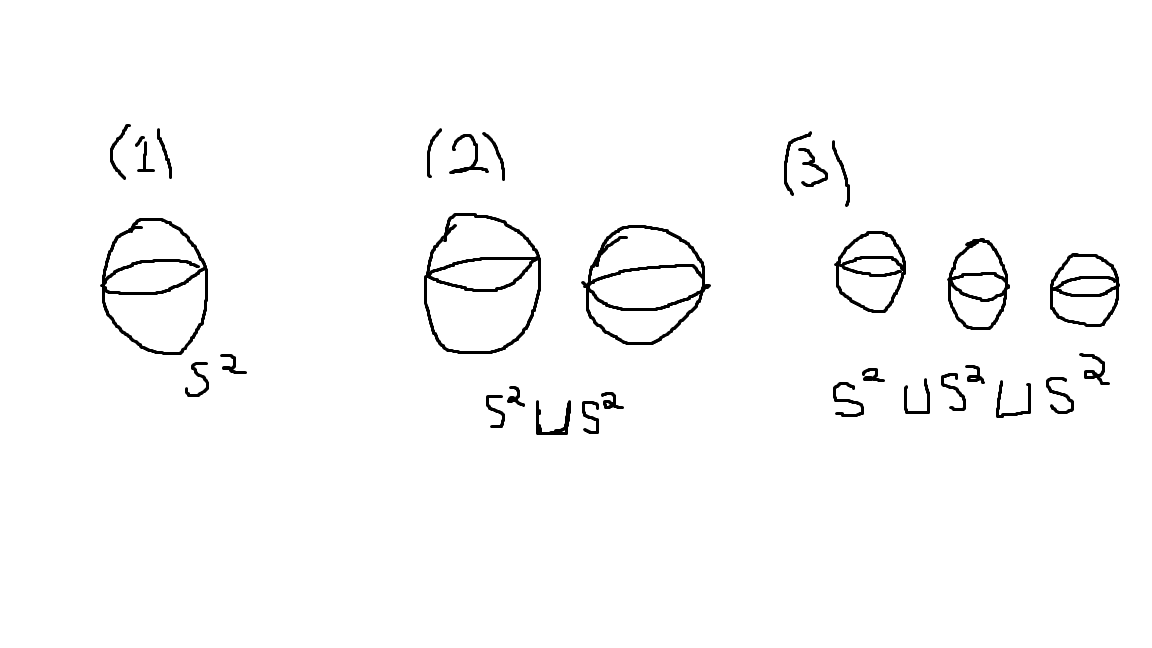
\includegraphics[width=0.90\linewidth]{Nondiffeomorphic.png}
        \end{figure}
        \qed
    \end{pb}
    \begin{pb}
        \textbf{(i)} Suppose they are compatible, then the transition map between charts \((\mathbb{R},\mathbb{R},1) \tand (\mathbb{R},\mathbb{R},g)\) is smooth, explicitly the transition map is given by \(g^{-1}\circ1 = g^{-1}\). This is a contradiction since \(g^{-1} = (x \mapsto \sqrt[3]{x})\) is not smooth at zero, since \(\lim_{x \to 0}\abs{\frac{\sqrt[3]{x} - 0}{x - 0}} = \lim_{x\to0}\abs{x^{-2/3}} = \infty\), so the function is not even differentiable at zero, this is a contradiction since transition functions are smooth.

        \textbf{(ii)} \(g: \mathbb{R}_\mathcal{A} \to \mathbb{R}_{g(\mathcal{A})}\) is the desired diffeomorphism. In order to check that \(g\) is smooth on charts, it suffices to check that \(g\) is smooth on the \((\mathbb{R},\mathbb{R},1) \tand (\mathbb{R},\mathbb{R},g)\) charts, because smoothness of transition functions allows us to map from any other chart by precomposing \(g\) with a transition map, and analogously to any chart by postcomposing \(g\) with a transition map. Thus the induced map on coordinates is \(g^{-1}\circ g\circ1 = 1\), the map \(1 = (x \mapsto x)\) is smooth. Using the same reasoning it suffices to check \(g^{-1}\) is smooth only on the charts \((\mathbb{R},\mathbb{R},g) \tand (\mathbb{R},\mathbb{R},1)\) where the induced map on coordinates is given by \(1\circ g^{-1}\circ g = 1\).

        \textbf{(iii)} In general if \(X\) is a smooth manifold with atlas \((U_\alpha,V_\alpha,\phi_\alpha)\) and \(g: X \to X\) is a smooth homeomorphism (but not a diffeomorphism), then \((U_\alpha,g(V_\alpha),g\circ\phi_\alpha)\) is an atlas for \(X\) (the only check needed is that \((g\circ\phi)_{\alpha \beta}\) is smooth, but \((g\circ\phi)_{\alpha \beta} = (g\circ\phi_\beta)^{-1}\circ(g\circ\phi_\alpha) = \phi_{\alpha \beta}\)). But it is also the case that these atlases are not compatible, since one of the transition maps would be \(\phi_\alpha\circ (g\circ\phi_\alpha)^{-1} = g^{-1}\) which is not smooth by assumption. However, it is the case that the smooth structures given by the two atlases are diffeomorphic via \(g: X_\mathcal{A} \to X_{g(\mathcal{A})}\), to check its a diffeomorphism, the maps between charts are of the form \((g\circ\phi_\beta)^{-1}g\circ\phi_\alpha = \phi_\beta^{-1}\circ\phi_\alpha\) and the maps between charts for the inverse are of the form \(\phi_\beta^{-1} \circ g^{-1}\circ(g\circ\phi_\alpha) = \phi_\beta^{-1}\circ\phi_\alpha\) both of which are smooth. \qed
    \end{pb}
    \begin{pb}
        \textbf{(i)} Assume first that \(k<j\), then
        \begin{align*}
            \phi_{jk}(x_1,\hdots,x_n) :&= \phi_k^{-1}\phi_j(x_1,\hdots,x_n) = \phi_k^{-1}[x_1:\cdots:x_{j-1}:1:x_j:\cdots:x_n] \\
            &= \phi_k^{-1}[x_1x_k^{-1}:\cdots:x_{j-1}x_k^{-1}:x_k^{-1}:x_jx_k^{-1}:\cdots:x_nx_k^{-1}] \\
            &= (x_1x_k^{-1},\hdots,x_{k-1}x_k^{-1},x_{k+1}x_k^{-1},\hdots,x_{j-1}x_k^{-1},x_k^{-1},x_jx_k^{-1},\hdots,x_nx_k^{-1})
        \end{align*}
        If \(j > k\), then
        \begin{align*}
            \phi_{jk}(x_1,\hdots,x_n) :&= \phi_k^{-1}\phi_j(x_1,\hdots,x_n) = \phi_k^{-1}[x_1:\cdots:x_{j-1}:1:x_j:\cdots:x_n] \\
            &= \phi_k^{-1}[x_1x_k^{-1}:\cdots:x_{j-1}x_k^{-1}:x_k^{-1}:x_jx_k^{-1}:\cdots:x_nx_k^{-1}] \\
            &= (x_1x_k^{-1},\hdots,x_{j-1}x_k^{-1},x_k^{-1},x_jx_k^{-1},\hdots,x_{k-2}x_k^{-1},1,x_{k+1}x_k^{-1},\hdots,x_nx_k^{-1})
        \end{align*}
        The transition function in each coordinate \((x_i) \mapsto x_k^{-1}\) is smooth on \(U_k\) and hence also \(U_k \cap U_j\) and the product of smooth functions is smooth (the coordinate and constant functions are always smooth).

        \textbf{(ii)} We take the map \(S^n/\sim_1 \to \mathbb{R}^{n+1}\setminus\set{0}/\sim_2\) by taking \([x]_1 \mapsto [x]_2\), since the two representatives of the same equivalence class in \(S^n/\sim_1\) differ by an element of \(\mathbb{R}^\times\) the map is well defined, this map is injective since two elements on the sphere differing by a constant multiple is only possible when the constant is \(\pm 1\), it is also surjective since very element of \(\mathbb{R}^{n+1}\setminus\set{0}\) is a multiple of an element on the unit sphere, thus the map is bijective and its clear in that case that the inverse is \([x]_2 \mapsto [x]_1\).  

        To see that its a homeomorphism consider the following diagrams with \(\iota\) denoting inclusion:
        \begin{equation*}
            \begin{tikzcd}
                S^n \arrow[r,"{\iota}"] \arrow[d,"{}"] &\mathbb{R}^{n+1}\setminus\set{0} \arrow[d,"{}"] \\
                S^n/\sim_1 \arrow[r,"{[x]_1\mapsto [x]_2} "] & \frac{\mathbb{R}^{n+1}\setminus\set{0}}{\sim_2}
            \end{tikzcd}
            \begin{tikzcd}
                S^n  \arrow[d,"{}"] &\mathbb{R}^{n+1}\setminus\set{0} \arrow[d,"{}"]\arrow[l,"{\frac{x}{\norm{x}} \leftarrow x}"] \\
                S^n/\sim_1  & \frac{\mathbb{R}^{n+1}\setminus\set{0}}{\sim_2} \arrow[l,"{[x]_1\leftarrow [x]_2} "]
            \end{tikzcd}
        \end{equation*}
        Since \(\iota\) and \(x \mapsto \frac{x}{\norm{x}}\) are continuous the diagrams show that \([x]_1 \mapsto [x]_2\) is a homeomorphism.
        
        to check that it induces a diffeomorphism we simply compute the transition maps and denote the transition maps in the class example as \(\varphi_j\) to avoid confusion. (assume \(j < k\))
        \begin{align*}
            \varphi_j^{-1}([x]_2 \mapsto [x]_1)\phi_k(x_1,\hdots,x_n) = \varphi_j^{-1}([x]_2 \mapsto [x]_1)[x_1:\cdots:x_{k-1}:1:x_k:\cdots:x_n]
        \end{align*}
        Now denoting \(\mathbf{x} = (x_1,\hdots,x_{k-1},1,x_k,\hdots,x_n)\), its immediate that \(\norm{\mathbf{x}} > 0\)
        \begin{align*}
            \varphi_j^{-1}([x]_2 \mapsto [x]_1)[x_1:\cdots:x_{k-1}:1:x_k:\cdots:x_n] &= \varphi_j^{-1}\left[\frac{x_1}{\norm{x}}:\cdots:\frac{x_{k-1}}{\norm{x}}:\frac{1}{\norm{x}}:\frac{x_k}{\norm{x}}:\cdots:\frac{x_n}{\norm{x}}\right] \\
            &= \text{sgn}(x_j)\left(\frac{x_1}{\norm{x}},\hdots,\widehat{\frac{x_j}{\norm{x}}},\hdots,\frac{x_{k-1}}{\norm{x}},\frac{1}{\norm{x}},\frac{x_k}{\norm{x}},\cdots,\frac{x_n}{\norm{x}}\right)
        \end{align*}
        This is smooth since \(\norm{\mathbf{x}} = \sqrt{1 + \sum_1^n x_i^2}\) is smooth, and since \(\frac{1}{x}\) is smooth away from zero (with the former being atleast 1) their composition is smooth, the fact that products of smooth functions are smooth finishes the proof that the map is smooth in each coordinate.

        \begin{align*}
            \phi_j^{-1}([x]_1 \mapsto [x]_2)\varphi_k(x_1,\hdots,x_n) &= \phi_j^{-1}([x]_2 \mapsto [x]_1)\left[x_1:\cdots:x_{k-1}:\sqrt{1-\sum_1^n x_i^2}:x_k:\cdots:x_n\right] \\
            &= \phi_j^{-1}\left[x_1:\cdots:x_{k-1}:\sqrt{1-\sum_1^n x_i^2}:x_k:\cdots:x_n\right] \\
            &= \phi_j^{-1}\left[x_1x_j^{-1}:\cdots:x_{k-1}x_j^{-1}:x_j^{-1}\sqrt{1-\sum_1^n x_i^2}:x_kx_j^{-1}:\cdots:x_nx_j^{-1}\right] \\
            &= \left(x_1x_j^{-1},\hdots,x_{j-1}x_j^{-1},x_{j+1}x_j^{-1},\hdots,x_{k-1}x_j^{-1},x_j^{-1}\sqrt{1 - \sum_1^n x_i^2},x_kx_j^{-1},\hdots,x_nx_j^{-1}\right)
        \end{align*}
        Since \(x_j \neq 0\) on \(\phi_j^{-1}(V_k) \subset V_j\), and \(x \mapsto \sqrt{x}\) is smooth on \((0,\infty)\) with \(\sum_1^n x_i^2 < 1\) we have that this map is smooth in each coordinate, which suffices to show its a diffeomorphism (here we are of courses using that products and compositions of smooth maps are smooth). This suffices to show the map is a diffeomorphism for \(j<k\), if \(j \geq k\) the computation is slightly different since a different factor gets dropped, but the coordinate functions are similar and still smooth. \qed
    \end{pb}
\end{document}